\section{A departure at a jump of the return arc}\label{app:td-jump}

The jump convention of Section~\ref{sec:td-core} decides the duration of a route whose schedule reaches a repeated abscissa exactly. Consider the customer sequence $\langle23,21,12,3,4,25,30,29\rangle$ on the TDVRP instance Rifki-30 of the Rifki2020 family, whose times are in seconds. A vehicle leaving the depot at 1341 is ready to leave customer~29 at exactly 2880, where the return arc $(29,0)$ stores 2 knots with the same abscissa. The first knot gives the arrival 3084, which is attained at that instant, while the second gives the upper ordinate 3126, from which the following piece starts (Figure~\ref{fig:rifki-depot-jump}).

\begin{figure}[htbp]
\centering
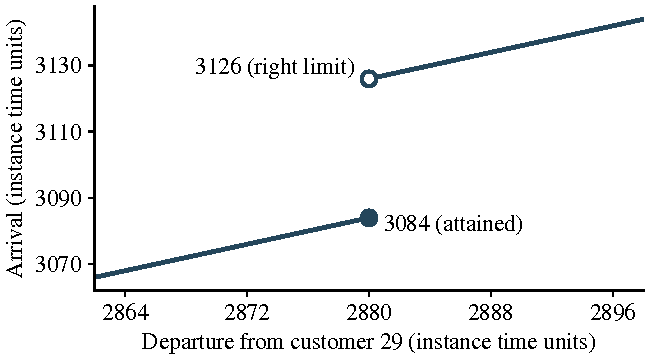
\includegraphics[width=11cm]{figures/rifki30-depot-jump.pdf}
\caption{Final arc $(29,0)$ of the Rifki-30 route near departure 2880. The filled point is the arrival attained at the repeated abscissa, and the open point marks the upper ordinate from which the next piece starts.}\label{fig:rifki-depot-jump}
\end{figure}

Under \id{td-binary64-exact-v1}, the vehicle therefore returns at 3084, and the route has duration $3084-1341=1743$. This value is also the minimum duration over all feasible depot departures, and 1341 is the earliest departure attaining it. A vehicle ready to leave customer~29 at any later time, however close to 2880, would instead follow the upper piece and return after 3126. Hence, an evaluation that rounds the ready time upwards by a single binary64 step crosses the jump and adds slightly more than 42 to the return time, which is why the exact profile keeps every intermediate time exact.
